\chapter{Benchmarking and Experiments}
\label{chapter5}
Introduce each domain, what makes it difficult, why it was chosen, etc. Show results from each domain, and discuss.
\citep{osband2020bsuite, 1606.01540}
\section{Deterministic Gridworld}
A simple gridworld, with a door that is open. The model embedded has a closed door.
\section{Stochastic Gridworld}
A simple gridworld, with a door that is open with probability 0.5, closed otherwise. The model embedded suggests that the door is closed with probability 1.0.
\section{Cliff-Walking}
\begin{figure}[h!]
    \centering
    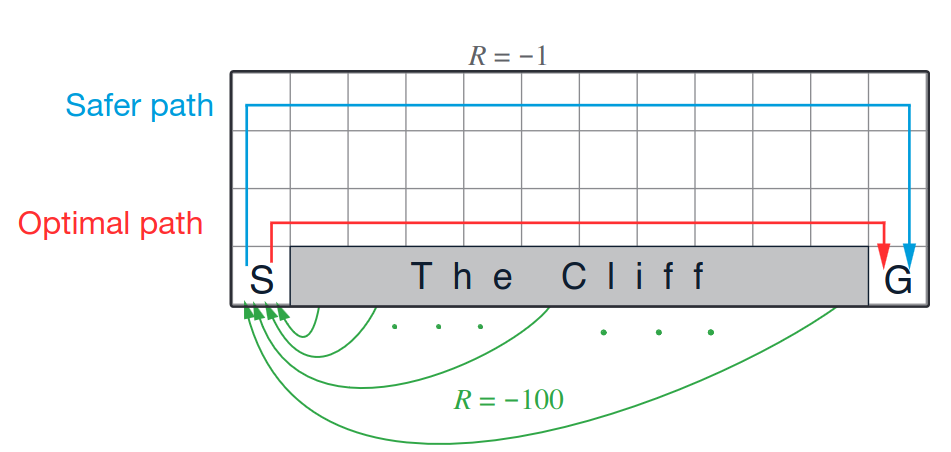
\includegraphics[max size={\textwidth}{\textheight}]{report/assets/envs/cliff-walking.png}
    \caption{Cliff-Walking Environment \citep{Sutton1998}}
    \label{fig:cliff-walking}
\end{figure}
\citep{1606.01540, Sutton1998}
\section{Windy Gridworld}
\begin{figure}[h!]
    \centering
    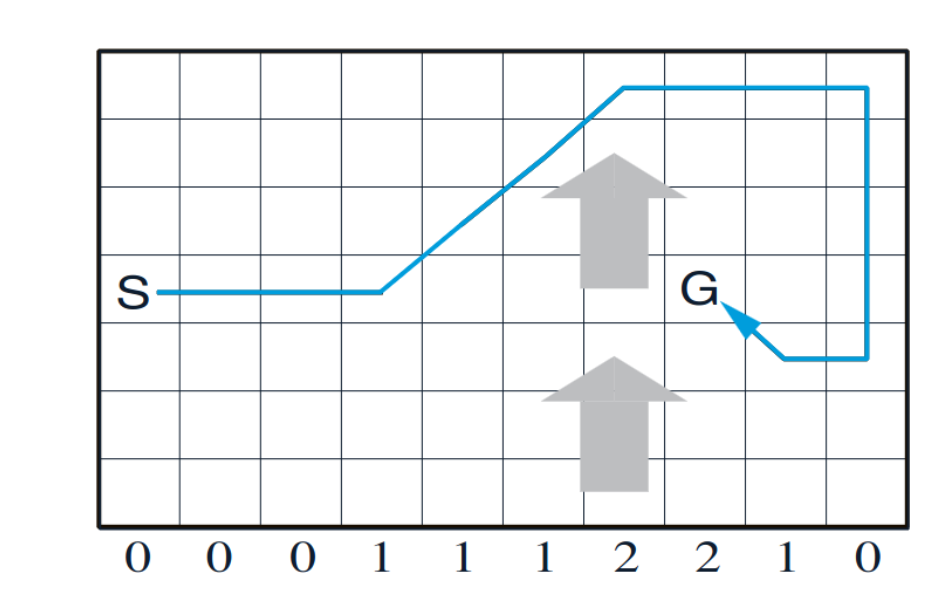
\includegraphics[max size={\textwidth}{\textheight}]{report/assets/envs/windy.png}
    \caption{Windy GridWorld Environment \citep{Sutton1998}}
    \label{fig:windy}
\end{figure}
\citep{Sutton1998}
\section{Stochastic Windy Gridworld}
\section{Frozen Lake}
\begin{figure}[h!]
    \centering
    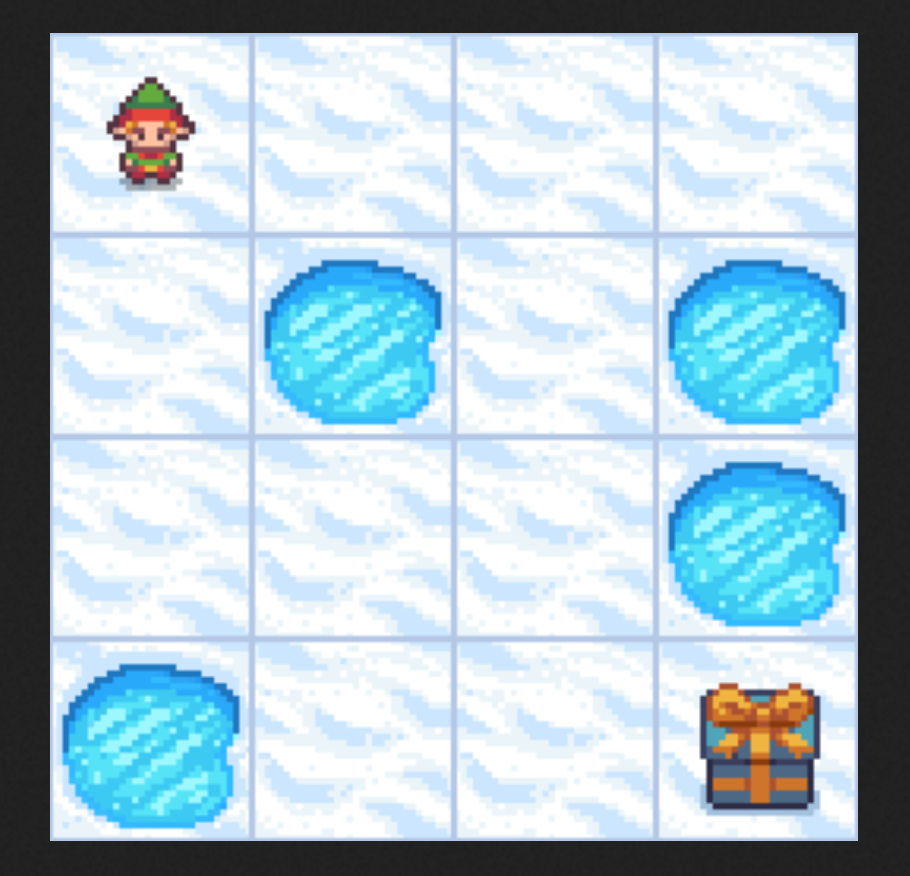
\includegraphics[max size={\textwidth}{\textheight}]{report/assets/envs/frozen-lake.png}
    \caption{Frozen Lake Environment \citep{1606.01540}}
    \label{fig:frozen}
\end{figure}
\citep{1606.01540}
\section{Discrete Cart-Pole}
\begin{figure}[h!]
    \centering
    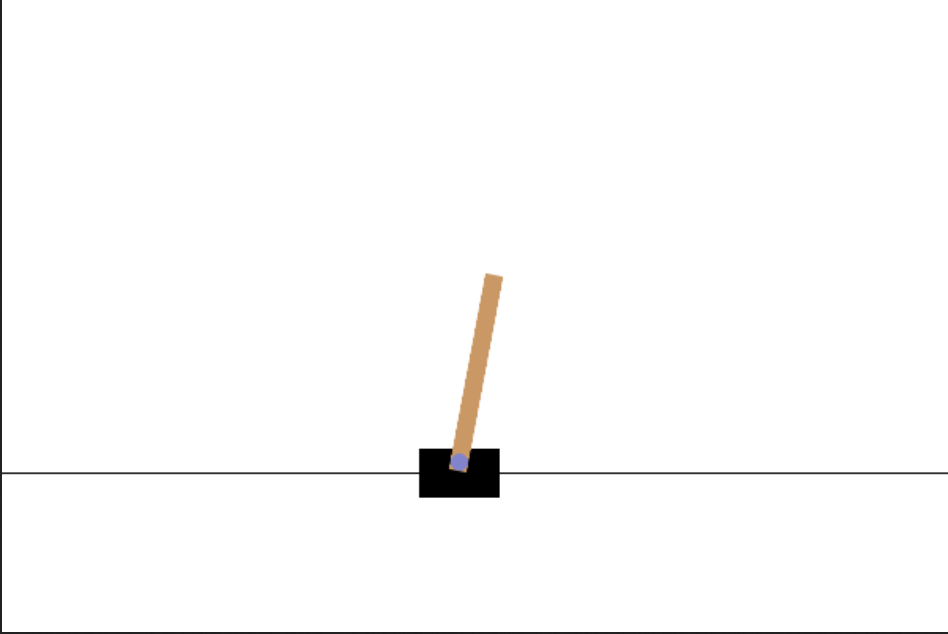
\includegraphics[max size={\textwidth}{\textheight}]{report/assets/envs/cartpole.png}
    \caption{CartPole Environment \citep{1606.01540, 6313077}}
    \label{fig:cartpole}
\end{figure}
\citep{1606.01540, 6313077}
\section{Discrete Mountain Car}
\begin{figure}[h!]
    \centering
    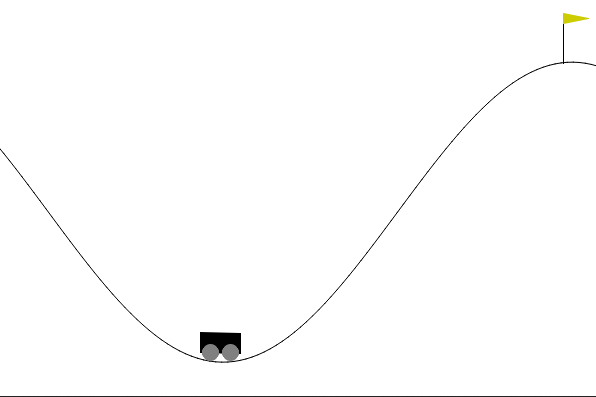
\includegraphics[max size={\textwidth}{\textheight}]{report/assets/envs/mountaincar.png}
    \caption{Mountain Car Environment \citep{1606.01540, Moore90efficientmemory-based}}
    \label{fig:cartpole}
\end{figure}
\citep{1606.01540, Moore90efficientmemory-based}